\documentclass[a4paper]{article}
\usepackage{fontspec}
\setmainfont{Times New Roman}[Ligatures=TeX]
\newfontfamily\cyrillicfont{Times New Roman}[Ligatures=TeX]
\IfFontExistsTF{JetBrains Mono}{
    \setmonofont{JetBrains Mono}
    \newfontfamily\cyrillicfonttt{JetBrains Mono}
}{
    \setmonofont{Courier New}
    \newfontfamily\cyrillicfonttt{Courier New}
}

\usepackage{polyglossia}
\setmainlanguage{russian}
\setotherlanguage{english}

\usepackage{geometry}
\geometry{
    a4paper,
    left=30mm,
    right=15mm,
    top=20mm,
    bottom=20mm,
}

% Межстрочный интервал и абзацы
\usepackage{setspace}
\onehalfspacing
\usepackage{indentfirst}
\setlength{\parindent}{1.25cm}
\emergencystretch=3em
\sloppy

\usepackage{fix-cm}
\renewcommand{\normalsize}{\fontsize{14pt}{21pt}\selectfont}

% Математика
\usepackage{amsmath, amssymb, amsthm}
\usepackage{mathtools}
\usepackage{tikz}
\usetikzlibrary{shapes, arrows, positioning, fit, calc}

% Теоремы
\theoremstyle{plain}
\newtheorem{theorem}{Теорема}[section]
\newtheorem{lemma}{Лемма}[section]
\newtheorem{corollary}{Следствие}[section]
\theoremstyle{definition}
\newtheorem{definition}{Определение}[section]

% Списки
\renewcommand{\labelitemi}{---}
\setlength{\leftmargini}{2cm}

% Таблицы и графика
\usepackage{array, booktabs, longtable}
\usepackage{graphicx}
\usepackage{float}
\usepackage[skip=10pt, labelfont=bf]{caption}
\captionsetup{labelsep=endash}
\renewcommand{\captionlabelfont}{\bfseries\fontsize{12pt}{18pt}\selectfont}
\renewcommand{\captionfont}{\fontsize{12pt}{18pt}\selectfont}
\renewcommand{\arraystretch}{1.15}

% Ссылки и оглавление
\usepackage[unicode, hidelinks]{hyperref}
\usepackage{nameref}

\addto\captionsrussian{
    \renewcommand{\contentsname}{СОДЕРЖАНИЕ}
    \renewcommand{\figurename}{Рисунок}
    \renewcommand{\tablename}{Таблица}
    \renewcommand{\lstlistingname}{Листинг}
    \renewcommand\refname{\hfill СПИСОК ИСПОЛЬЗОВАННЫХ ИСТОЧНИКОВ \hfill}
}

% Заголовки
\makeatletter
\renewcommand{\@seccntformat}[1]{\csname the#1\endcsname.\quad}
\renewcommand\section{\@startsection {section}{1}{\z@}%
    {-3.5ex \@plus -1ex \@minus -.2ex}%
    {2.3ex \@plus.2ex}%
    {\centering\normalfont\bfseries\fontsize{16pt}{24pt}\selectfont}}
\renewcommand\subsection{\@startsection {subsection}{2}{\z@}%
    {-3.25ex\@plus -1ex \@minus -.2ex}%
    {1.5ex \@plus .2ex}%
    {\centering\normalfont\bfseries\fontsize{16pt}{24pt}\selectfont}}
\makeatother

% Библиография
\makeatletter
\renewcommand\@biblabel[1]{#1.}
\makeatother
\usepackage{url}

% Листинг
\usepackage{xcolor}
\usepackage{listings}

\definecolor{codegreen}{rgb}{0,0.6,0}
\definecolor{codeblue}{rgb}{0,0,0.8}
\definecolor{codered}{rgb}{0.8,0,0}

\lstset{
    basicstyle=\ttfamily\small,
    backgroundcolor=\color{white},
    frame=lines,
    rulecolor=\color{black},
    framerule=0.5pt,
    breaklines=true,
    breakatwhitespace=true,
    breakindent=20pt,
    numbers=left,
    numberstyle=\tiny\color{gray},
    stepnumber=1,
    numbersep=5pt,
    inputencoding=utf8,
    extendedchars=true,
    literate={},
    tabsize=4,
    showspaces=false,
    showstringspaces=false,
    showtabs=false,
    captionpos=t,
    belowcaptionskip=5pt,
    commentstyle=\color{codegreen},
    keywordstyle=\color{codeblue},
    stringstyle=\color{codered},
    identifierstyle=\color{black},
}


\begin{document}

\begin{center}
    \tableofcontents
\end{center}
\newpage

\phantomsection
\section*{ВВЕДЕНИЕ}
\addcontentsline{toc}{section}{ВВЕДЕНИЕ}

Нейронный машинный перевод (далее NMT) --- одна из основных задач обработки естественного языка.
С практической точки зрения он заключается в построении модели, которая по тексту на исходном языке формирует текст на целевом языке, сохраняя смысл, грамматическую корректность и контекст высказывания.
Наряду с классическими encoder-decoder системами на основе Transformer все чаще рассматриваются decoder-only языковые модели и архитектуры с линейной обработкой последовательностей.
Результаты последних соревнований WMT показывают, что крупные языковые модели уже стали важной частью систем машинного перевода, однако специализированные NMT-модели по-прежнему остаются конкурентоспособными при контролируемом обучении на параллельных корпусах~\cite{wmt24_general}.

Построение системы NMT включает выбор архитектуры модели, способа представления исходного и целевого текста, схемы организации перевода, набора языковых направлений, состава обучающих данных и метода обучения.
Эти решения совместно определяют качество перевода, вычислительную сложность и возможность переноса модели на новые языки или домены.

С момента появления NMT было предложено несколько основных архитектурных подходов.
К классическим решениям относятся рекуррентные модели LSTM с механизмом внимания~\cite{luong}.
Позднее основой большинства систем стали модели Transformer с механизмом самовнимания~\cite{transformer}.
В последние годы также развиваются архитектуры, основанные на моделях пространства состояний, в частности Mamba~\cite{mamba}.
Эти подходы по-разному работают с контекстом, поэтому их имеет смысл сравнивать не только по качеству перевода, но и по ограничениям при обработке длинных последовательностей.

Не менее важна схема организации самой модели перевода.
В классическом варианте encoder-decoder encoder строит представление исходного предложения, а decoder по этому представлению формирует перевод.
В decoder-only подходе исходный текст и целевой перевод рассматриваются как части одной авторегрессионной последовательности.
Эти схемы могут использоваться с разными архитектурами, поэтому сравнение архитектур без учета способа организации модели дает неполную картину.

Также отличаться может и языковой охват модели.
Модель может обучаться для одного направления перевода, например с одного фиксированного исходного языка на один целевой язык.
Другой вариант --- мультиязычная модель, которая работает сразу с несколькими языками и направлениями перевода.
Мультиязычные модели используют общие представления между языками, но одновременно требуют более сложной балансировки данных, постановки обучения и потенциально другой логики построения перевода.

Современные работы по машинному переводу также показывают, что качество обучающих данных становится не менее важным фактором, чем выбор архитектуры~\cite{newspalm_data}.
Шумные параллельные пары, неверно определенный язык, неполные переводы и технические фрагменты могут ухудшать обучение даже крупных моделей.
Поэтому подготовка корпуса должна рассматриваться как часть общей системы NMT, а не как вспомогательный этап.
Количество техник работы с данными и их комбинаций в переводе велико: фильтрация шумных параллельных предложений, удаление дубликатов, ограничения по длине и соотношению длин предложений, различные способы аугментации данных или генерирование синтетических данных.

Различаются и подходы к обучению моделей перевода.
Базовый вариант --- supervised learning, при котором модель обучается на парах исходных предложений и эталонных переводов.
Дополнительно могут использоваться методы дообучения с учетом автоматических метрик, человеческих оценок или reinforcement learning.
Задача исследования состоит не только в описании отдельных моделей, но и в сопоставлении архитектурных, языковых, корпусных и обучающих решений в общей постановке нейронного машинного перевода.

\subsection*{Постановка задачи}
Целью работы является сравнительное исследование подходов к построению и обучению моделей NMT.
Для достижения поставленной цели необходимо решить следующие задачи:
\begin{enumerate}[label=\arabic*)]
	\item рассмотреть общую постановку задачи NMT;
	\item рассмотреть подходы к подготовке, фильтрации и аугментации обучающих данных;
	\item описать основные подходы к обучению, подбору гиперпараметров и оценке качества моделей перевода;
	\item сравнить архитектуры LSTM, Transformer и Mamba в задачах перевода;
	\item охарактеризовать однонаправленные и мультиязычные модели перевода;
	\item сопоставить encoder-decoder и decoder-only схемы;
\end{enumerate}

\newpage
\section{MAMBA-МОДЕЛИ В МАШИННОМ ПЕРЕВОДЕ}

\subsection{Машинный перевод как задача моделирования последовательностей}

Нейронный машинный перевод обычно формулируется как задача условного языкового моделирования.
Пусть исходное предложение задано последовательностью токенов
$x = (x_1, \ldots, x_m)$, а перевод --- последовательностью
$y = (y_1, \ldots, y_n)$.
Тогда модель должна оценивать вероятность перевода
\begin{equation}
    p(y \mid x) = \prod_{t=1}^{n} p(y_t \mid y_{<t}, x).
\end{equation}

На практике для такой задачи часто используют архитектуру encoder-decoder.
Encoder преобразует исходную последовательность в набор скрытых представлений, а decoder по этим представлениям авторегрессионно строит перевод.
В качестве базовой рекуррентной модели в данной работе используется LSTM с механизмом внимания Лионга \cite{luong}.
Такой выбор позволяет сравнить современные архитектуры с классическим подходом к машинному переводу.

Задачу sequence-to-sequence можно сформулировать и без отдельного encoder.
В decoder-only подходе исходное предложение, служебный разделитель и целевой перевод объединяются в одну последовательность.
Модель обучается как языковая модель, то есть предсказывает следующий токен по предыдущим токенам, но функция потерь учитывается только на токенах перевода.
В этом случае исходное предложение играет роль префикса, который задает условие для генерации.
Такая схема используется в современных авторегрессионных языковых моделях и позволяет строить перевод одной моделью без явного разделения на encoder и decoder.

В рекуррентной модели скрытое состояние обновляется последовательно.
В самом общем виде это можно записать так:
\begin{equation}
    h_t = f(h_{t-1}, x_t), \qquad y_t = g(h_t).
\end{equation}
Именно наличие состояния делает LSTM и Mamba близкими по общей идее: обе модели накапливают информацию о прошлых токенах.
Различие заключается в том, как это состояние параметризуется и насколько эффективно его можно вычислять при обучении.

\subsection{Механизм внимания и Transformer}

Модели Transformer стали основой многих современных систем машинного перевода \cite{transformer}.
Их ключевой компонент --- механизм самовнимания, который позволяет каждому токену напрямую учитывать другие токены последовательности.
Для матриц запросов $Q$, ключей $K$ и значений $V$ самовнимание записывается следующим образом:
\begin{equation}
    \operatorname{Attention}(Q, K, V) =
    \operatorname{softmax}\left(\frac{QK^T}{\sqrt{d}}\right)V,
\end{equation}
где $d$ --- размерность векторов ключей.

В encoder-decoder Transformer encoder строит контекстные представления исходного предложения, а decoder использует два вида внимания: причинное самовнимание по уже сгенерированным токенам и внимание к выходам encoder.
Такой подход хорошо работает в машинном переводе, но самовнимание требует попарного сравнения токенов.
Поэтому вычислительная сложность и расход памяти растут квадратично по длине последовательности.
Это ограничение особенно заметно при работе с длинными текстами.

\subsection{Mamba и модели пространства состояний}

Mamba относится к моделям, которые используют скрытое состояние для обработки последовательности \cite{mamba}.
Базовую идею удобно описать через дискретную модель пространства состояний:
\begin{equation}
    \begin{gathered}
        h_t = \bar{A}h_{t-1} + \bar{B}x_t, \\
        y_t = Ch_t + Dx_t,
    \end{gathered}
\end{equation}
где $h_t$ --- скрытое состояние, $x_t$ --- входной токен, $y_t$ --- выход, а матрицы $\bar{A}$, $\bar{B}$, $C$ и $D$ задают обновление состояния и построение выхода.
Если эти параметры фиксированы для всех токенов, модель одинаково обрабатывает все позиции последовательности.
Это удобно для вычислений, но ограничивает способность модели избирательно запоминать важные элементы текста.

Mamba решает эту проблему за счет входозависимых параметров.
Для каждого токена строятся свои значения $\Delta_t$, $B_t$ и $C_t$:
\begin{equation}
    [\delta_t, B_t, C_t] = W_x x_t + b_x, \qquad
    \Delta_t = \operatorname{softplus}(W_{\Delta}\delta_t + b_{\Delta}).
\end{equation}
После этого состояние обновляется по правилу
\begin{equation}
    h_t = \bar{A}_t h_{t-1} + \bar{B}_t x_t, \qquad
    y_t = C_t h_t + D x_t,
\end{equation}
где $\bar{A}_t$ и $\bar{B}_t$ зависят от $\Delta_t$.
Благодаря этому модель может по-разному обрабатывать разные токены: одни сохранять в состоянии, а другие быстро забывать.

Из-за входозависимых параметров Mamba нельзя заранее представить как одну фиксированную свертку.
Тем не менее модель остается быстрой благодаря selective scan --- параллельному сканированию, которое выполняет рекуррентные обновления за линейное время и эффективно использует современные графические ускорители.
Псевдокод блока Mamba приведен в листинге \ref{listing:mamba_pseudocode}.

\begin{lstlisting}[language=Python, caption={Основные операции блока Mamba}, label={listing:mamba_pseudocode}]
Input: x : (B, L, D)
Parameters: A : (D, N)

x, z : (B, L, E * D) <- Linear_in(x)
x : (B, L, E * D) <- SiLU(CausalConv1D(x))

B : (B, L, N) <- s_B(x)
C : (B, L, N) <- s_C(x)
Delta : (B, L, E * D) <- softplus(Parameter + s_Delta(x))

A_bar, B_bar <- discretize(Delta, A, B)
y : (B, L, E * D) <- selective_scan(A_bar, B_bar, C)(x)
y <- y * SiLU(z)

Output: Linear_out(y)
\end{lstlisting}

Для машинного перевода это свойство важно, потому что не все токены одинаково значимы для построения перевода.
Имена собственные, глаголы и числовые значения часто нужно сохранять точнее, чем служебные слова или отдельные знаки препинания.
Поэтому избирательное обновление состояния может быть полезной альтернативой полному самовниманию.

\subsection{Mamba только с декодером}

В классической схеме encoder-decoder исходное предложение и перевод обрабатываются разными частями модели.
В Mamba только с декодером эта граница задается не архитектурой, а форматом последовательности.
Исходное предложение, разделитель и перевод объединяются в один авторегрессионный контекст:
\begin{equation}
    z = (x_1, \ldots, x_m, \operatorname{sep}, y_1, \ldots, y_n).
\end{equation}
Тогда условная вероятность перевода записывается как
\begin{equation}
    p(y \mid x) = \prod_{t=1}^{n}
    p(y_t \mid x_1, \ldots, x_m, \operatorname{sep}, y_{<t}).
\end{equation}

При обучении модель предсказывает следующий токен для всей объединенной последовательности, но ошибка учитывается только на части, соответствующей переводу:
\begin{equation}
    \mathcal{L} = - \sum_{t=1}^{n}
    \log p(y_t \mid x_1, \ldots, x_m, \operatorname{sep}, y_{<t}).
\end{equation}
Во время генерации исходное предложение и разделитель подаются как префикс, после чего модель последовательно добавляет токены перевода.

Такой подход хорошо согласуется с причинной природой Mamba: состояние после обработки исходного предложения становится сжатым представлением условия для дальнейшей генерации.
Преимущество decoder-only схемы состоит в единой авторегрессионной постановке задачи и более простой структуре модели.
Ограничение состоит в том, что связь с исходным предложением проходит через общий последовательный контекст, а не через отдельный слой внимания к выходам encoder.

\newpage
\IfFileExists{.__texlab_dummy}{\bibliography{../texlab_refs}}{}

\section{РЕАЛИЗАЦИЯ И АНАЛИЗ ЭФФЕКТИВНОСТИ МОДЕЛЕЙ}

В практической части работы были реализованы и обучены четыре модели нейронного машинного перевода: LSTM с механизмом внимания, Transformer, Mamba в схеме encoder-decoder и Mamba только с декодером.
LSTM использовалась как базовая рекуррентная модель.
Transformer был выбран как стандартная архитектура машинного перевода с механизмом самовнимания.
Две модели Mamba позволяют сравнить классическую encoder-decoder схему с decoder-only подходом.
Такое сравнение актуально, поскольку Mamba рассматривается как альтернатива self-attention для обработки длинного контекста без квадратичной сложности~\cite{transformer,mtssm}.

Реализация выполнена на языке Python с использованием библиотеки \textbf{PyTorch}.
Для всех моделей использовалась одинаковая схема обучения.
Модели обучались с оптимизатором AdamW, ограничением нормы градиента и функцией потерь cross-entropy с label smoothing.
Планировщик скорости обучения состоял из линейного warmup и последующего косинусного убывания.

Для обучения использовался вычислительный стенд с видеокартой NVIDIA-H100.

\subsection{Датасет и предобработка данных}

Для обучения использовалась русско-английская часть датасета OPUS-100~\cite{opus100}.
OPUS-100 является многоязычным параллельным корпусом, собранным на основе открытых корпусов OPUS.
Русско-английская часть содержит около 1 млн параллельных пар.
Каждый пример датасета представляет собой пару предложений: предложение на русском языке и соответствующий ему перевод на английский язык.

В работе использовались стандартные разбиения датасета на обучающую, валидационную и тестовую части.
Во время обучения длина последовательности ограничивалась 256 токенами.
Такая граница отсекает слишком длинные предложения, которые сильно увеличивают расход памяти, но при этом сохраняет большую часть обычных предложений корпуса.

Для дополнительного контроля качества данных применялись две проверки.
Во-первых, автоматически проверялся язык предложений.
Так выявлялись примеры, где в русской колонке находился не русский текст или наоборот.
Во-вторых, для части пар оценивалась семантическая близость предложений.
Такая проверка нужна потому, что параллельные корпуса могут содержать технический шум: неполные переводы, перепутанные строки, одинаковые предложения на разных языках.

\subsection{Токенизатор}

Для токенизации использовалась subword-модель Unigram~\cite{sentencepiece}.
В отличие от простого разбиения по словам, subword-токенизация позволяет работать с неизвестными словами, редкими формами и морфологически богатыми языками.
Это особенно важно для русского языка, где одно и то же слово может иметь много грамматических форм.

Перед обучением словаря выполнялась нормализация Unicode в форме NFKC.
Далее применялась предварительная токенизация:
\begin{itemize}
    \item пробелы кодировались через metaspace-представление;
    \item знаки препинания выделялись в отдельные токены;
    \item числа разбивались на отдельные цифровые токены.
\end{itemize}

Отдельная обработка чисел и пунктуации важна для перевода.
Числа чаще всего должны переноситься в перевод без изменения, а знаки препинания задают структуру предложения.
Если такие элементы смешивать с соседними словами, модели сложнее научиться переносить их корректно.

Для encoder-decoder моделей использовались специальные токены начала и конца последовательности, padding-токен и токен неизвестного фрагмента.
Для модели только с декодером дополнительно использовался разделитель между исходным предложением и переводом.

\subsection{Используемые метрики}

Качество машинного перевода нельзя надежно оценивать только функцией потерь, поэтому основной метрикой качества в работе является BLEU.
Метрика BLEU сравнивает $n$-граммы машинного перевода с $n$-граммами эталонного перевода~\cite{bleu}:
\begin{equation}
    \operatorname{BLEU} = BP \cdot \exp\left(\sum_{n=1}^{N} w_n \log p_n\right),
\end{equation}
где $p_n$ --- модифицированная точность по $n$-граммам, $w_n$ --- веса, а $BP$ --- штраф за слишком короткий перевод.
В работе BLEU вычислялся с помощью библиотеки SacreBLEU~\cite{sacrebleu}.

Дополнительно учитывалось число параметров модели.
Эта величина важна, потому что две модели с близким качеством перевода могут существенно отличаться по требованиям к памяти и скорости обучения.

\subsection{Архитектуры моделей}

Первой моделью была LSTM encoder-decoder с механизмом внимания.
Encoder является двунаправленным: одна LSTM читает исходное предложение слева направо, вторая --- справа налево.
Decoder генерирует перевод авторегрессионно.
На каждом шаге применяется механизм внимания, который строит контекстный вектор по скрытым состояниям encoder.

Вторая модель построена на архитектуре Transformer.
Encoder использует самовнимание для построения представлений исходного предложения.
Decoder применяет причинное самовнимание к уже сгенерированной части перевода и отдельный слой внимания к выходам encoder.
Эта модель служит сильной нейросетевой базой для сравнения с Mamba.

Третья модель использует Mamba-блоки в схеме encoder-decoder.
В encoder и decoder последовательная обработка выполняется Mamba-блоками, а связь между исходным предложением и переводом задается слоем внимания.
Такой вариант сохраняет привычную для машинного перевода структуру encoder-decoder, но заменяет часть последовательной обработки на блоки Mamba.

Четвертая модель --- Mamba только с декодером.
В этой схеме исходное предложение и перевод рассматриваются как одна авторегрессионная последовательность.
Во время обучения модель получает исходный текст и правильный перевод, но ошибка оптимизации считается только по токенам перевода.
Во время вывода исходное предложение задает префикс, после чего модель продолжает последовательность токенами перевода.

В таблице \ref{tab:configs} приведены основные конфигурации моделей.

\begin{table}[H]
    \centering
    \caption{Основные конфигурации моделей}
    \label{tab:configs}
    \resizebox{0.98\textwidth}{!}{%
    \begin{tabular}{|l|c|c|c|c|}
        \hline
        Модель & Схема & Размер представления & Число слоев & Особенность \\
        \hline
        LSTM & encoder-decoder & 384 & 4 & рекуррентная базовая модель \\
        Transformer & encoder-decoder & 768 & 6+6 & самовнимание и слой внимания к encoder \\
        Mamba & encoder-decoder & 768 & 6+6 & Mamba-блоки и слой внимания к encoder \\
        Mamba decoder-only & только декодер & 512 & 8 & единая авторегрессионная последовательность \\
        \hline
    \end{tabular}}
\end{table}

\subsection{Графики обучения}

Все модели обучались на 100 тыс. итераций с размером батча 100.
Для BLEU использовались 40 проверок на валидационной выборке.

На рисунке \ref{fig:train_loss} показано изменение функции потерь на обучении.
У всех моделей значение функции потерь убывает, что говорит о корректном ходе оптимизации.
Transformer и Mamba в схеме encoder-decoder быстрее достигают меньших значений функции потерь, а LSTM и Mamba только с декодером сходятся более плавно.

\begin{figure}[H]
    \centering
    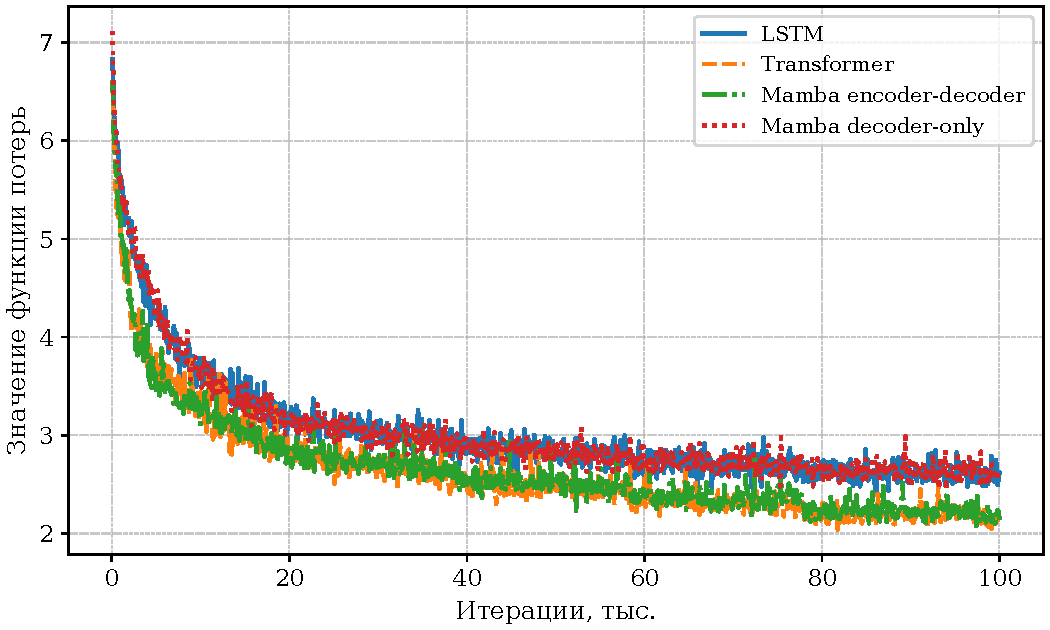
\includegraphics[width=0.88\textwidth]{images/train_loss_successful.pdf}
    \caption{Изменение функции потерь на обучении}
    \label{fig:train_loss}
\end{figure}

На рисунке \ref{fig:validation_bleu} приведено изменение BLEU на валидационной выборке.
По этому графику видно, что Transformer и Mamba encoder-decoder дают близкое качество и заметно превосходят LSTM.
Mamba только с декодером набирает качество медленнее и в данном эксперименте уступает encoder-decoder вариантам.

\begin{figure}[H]
    \centering
    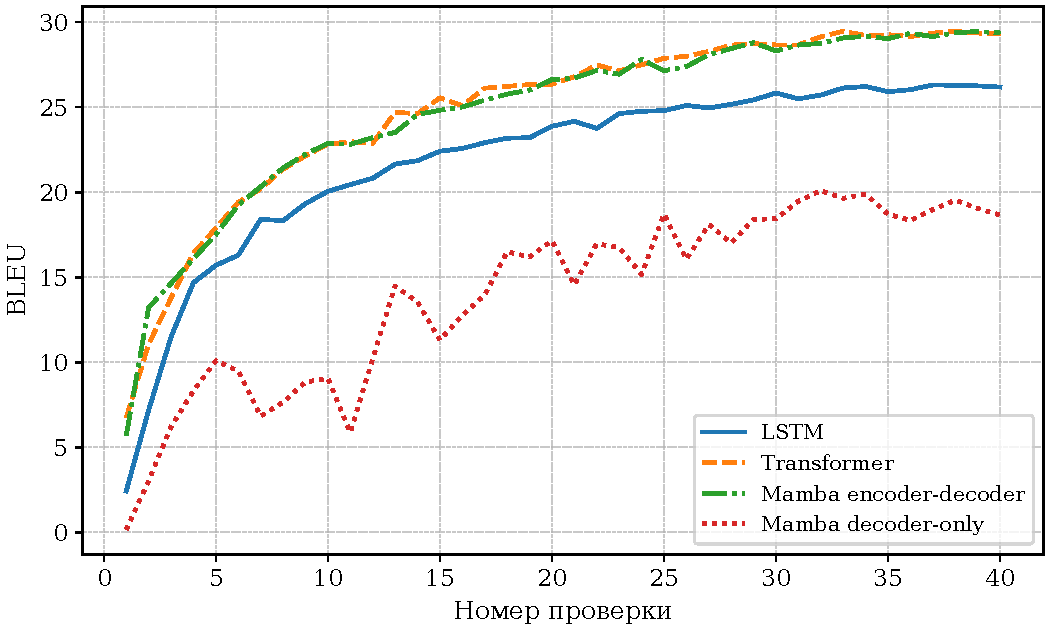
\includegraphics[width=0.88\textwidth]{images/validation_bleu_successful.pdf}
    \caption{Изменение BLEU на валидационной выборке}
    \label{fig:validation_bleu}
\end{figure}

\subsection{Итоговое сравнение}

Итоговые результаты представлены в таблице \ref{tab:results}.
Для BLEU указано лучшее значение на валидационной выборке.
Размер модели указан в миллионах параметров.

\begin{table}[H]
    \centering
    \caption{Итоговое сравнение моделей машинного перевода}
    \label{tab:results}
    \begin{tabular}{|l|c|c|}
        \hline
        Модель & BLEU & Число параметров \\
        \hline
        LSTM & 26.31 & 73.5M \\
        Transformer & 29.47 & 158.8M \\
        Mamba encoder-decoder & 29.45 & 190.3M \\
        Mamba decoder-only & 20.09 & 90.0M \\
        \hline
    \end{tabular}
\end{table}

По результатам видно, что Mamba в схеме encoder-decoder достигает качества, близкого к Transformer, и превосходит LSTM.
При этом вариант Mamba только с декодером показал более низкое значение BLEU.
Это означает, что для рассматриваемого корпуса явное разделение исходного предложения и перевода в encoder-decoder схеме оказалось полезным.
Тем не менее decoder-only вариант остается важным для сравнения, поскольку он показывает, как Mamba работает в единой авторегрессионной постановке задачи.

\newpage
\section*{ЗАКЛЮЧЕНИЕ}
\addcontentsline{toc}{section}{\protect ЗАКЛЮЧЕНИЕ}

В результате работы была изучена архитектура Mamba применительно к задаче нейронного машинного перевода.
Были рассмотрены две постановки sequence-to-sequence задачи: классическая схема encoder-decoder и модель только с декодером, где исходное предложение и перевод образуют одну авторегрессионную последовательность.
Также была кратко описана связь Mamba с моделями пространства состояний и идея избирательного обновления скрытого состояния.

В практической части были обучены и сравнены четыре модели: LSTM с механизмом внимания, Transformer, Mamba encoder-decoder и Mamba decoder-only.
Основной метрикой качества была BLEU, дополнительно учитывалось число параметров.
На русско-английском корпусе OPUS-100 Mamba в схеме encoder-decoder показала качество, близкое к Transformer, и превзошла LSTM.

Модель Mamba только с декодером уступила encoder-decoder вариантам по BLEU.
Это показывает, что для данной задачи явное кодирование исходного предложения остается полезным.
В то же время decoder-only схема работоспособна и может рассматриваться как отдельное направление для дальнейшего улучшения Mamba-моделей машинного перевода.

\newpage
\addcontentsline{toc}{section}{\protect СПИСОК ИСПОЛЬЗОВАННЫХ ИСТОЧНИКОВ}
\sloppy
\begin{thebibliography}{}
    \bibitem{luong}
    Luong M.-T., Pham H., Manning C.D.
    Effective Approaches to Attention-based Neural Machine Translation [Электронный ресурс]. — 2015. — URL: \detokenize{https://arxiv.org/abs/1508.04025}

    \bibitem{transformer}
    Vaswani A., Shazeer N., Parmar N., Uszkoreit J., Jones L., Gomez A.N., Kaiser Ł., Polosukhin I.
    Attention Is All You Need [Электронный ресурс]. — 2017. — URL: \detokenize{https://arxiv.org/abs/1706.03762}

    \bibitem{mamba}
    Gu A., Dao T.
    Mamba: Linear-Time Sequence Modeling with Selective State Spaces [Электронный ресурс]. — 2023. — URL: \detokenize{https://arxiv.org/abs/2312.00752}

    \bibitem{mtssm}
    Pitorro R., et al.
    How Effective Are State Space Models for Machine Translation? [Электронный ресурс]. — 2024. — URL: \detokenize{https://arxiv.org/abs/2402.18637}

    \bibitem{opus100}
    Zhang B., Williams P., Titov I., Sennrich R.
    Improving Massively Multilingual Neural Machine Translation and Zero-Shot Translation [Электронный ресурс]. — 2020. — URL: \detokenize{https://arxiv.org/abs/2004.11867}

    \bibitem{sentencepiece}
    Kudo T., Richardson J.
    SentencePiece: A simple and language independent subword tokenizer and detokenizer for Neural Text Processing [Электронный ресурс]. — 2018. — URL: \detokenize{https://arxiv.org/abs/1808.06226}

    \bibitem{bleu}
    Papineni K., Roukos S., Ward T., Zhu W.-J.
    BLEU: a Method for Automatic Evaluation of Machine Translation [Электронный ресурс] // Proceedings of ACL. — 2002. — URL: \detokenize{https://aclanthology.org/P02-1040/}

    \bibitem{sacrebleu}
    Post M.
    A Call for Clarity in Reporting BLEU Scores [Электронный ресурс] // Proceedings of WMT. — 2018. — URL: \detokenize{https://aclanthology.org/W18-6319/}
\end{thebibliography}

\newpage
\section*{ПРИЛОЖЕНИЕ А}
\addcontentsline{toc}{section}{\protect ПРИЛОЖЕНИЕ А}

В приложении приведены фрагменты реализации, использованные в работе.

\lstinputlisting[language=Python,caption={Фрагмент реализации LSTM с механизмом внимания},label={listing:lstm_impl}]{listings/luong_attention.py}
\newpage

\lstinputlisting[language=Python,caption={Фрагмент реализации блока Mamba},label={listing:mamba_impl}]{listings/mamba_mixer.py}
\newpage

\lstinputlisting[language=Python,caption={Фрагмент реализации Mamba только с декодером},label={listing:mamba_decoder_impl}]{listings/mamba_decoder.py}


\end{document}
